\subsection{Principle of operation of the TLP-HMM}

% Principle of operation
Later in this document, the new generator is referred as TLP-HMM.
The TLP-HMM requires two additional modules to be connected at each extremity of a classic 100ns \gls{tlp}.
These modules are simply referred hereafter as the \textit{absorber} and the \textit{shaping filter} (Fig. \ref{fig:tlp_hmm_architecture}).
The principle of the TLP-HMM is to re-route parts of an incoming rectangular pulse into the ground.
The remaining current is injected on a 2\textOmega{} calibration resistor, resulting in the same waveform than expected by the standards.
The role of each module is detailed in the following sections.

\begin{figure}[!h]
  \centering
  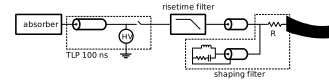
\includegraphics[width=0.9\textwidth]{src/5/figures/beges_tlp_hmm.pdf}
  \caption{TLP-HMM architecture}
  \label{fig:tlp_hmm_architecture}
\end{figure}

\subsubsection{Shaping filter}

% Role of the shaping filter
The shaping filter (see Fig. \ref{fig:shaping_filter_example}) deviates a part of the incoming rectangular pulse into the grounded coaxial shielding.
It is constituted of five different elements, an RLC network, a delay cable and an injection resistor.
The capacitor C is separated from the main propagation path by a small transmission line of delay \textDelta{}t.
The inductor L is neglected in this first part of the analysis.
It behaves as an open circuit at the beginning of the pulse.
The short coaxial cable creates a delay \textDelta{}t between the main line and the RLC network.
The injection resistor R\textsubscript{S} serves to increase the output impedance, in order to get closer to the behavior of an actual HMM generator.

\begin{figure}[!h]
  \centering
  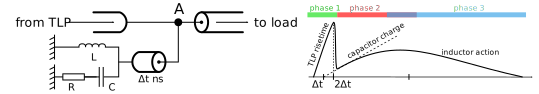
\includegraphics[width=0.98\textwidth]{src/5/figures/example_tlp_hmm.pdf}
  \caption{Shaping filter architecture and operation}
  \label{fig:shaping_filter_example}
\end{figure}

% Behavior of the filter - C
An example case is given to detail the behavior of the generator, with a focus on the shaping filter.
In phase 1 (graph on the right in Fig. \ref{fig:shaping_filter_example}), a \gls{tlp} is injected on the main line.
It reaches point A at $t=0$ and the voltage at A rises from 0 V.
The capacitor is still not visible from A and does not see the TLP rising edge yet.
At $t=\Delta t$, the pulse reaches the capacitor, which begins to charge.
This change in voltage and current in the capacitor branch is not visible immediately from point A until it propagates back.
Point A keeps rising with the TLP impulse until $t=2\Delta t$.
At this moment, potential at point A falls almost immediately to 0V, because the capacitor is drawing all the current, and its potential is low.
This results in the generation of the first peak.
The peak width is approximately $2\Delta t$.

% Behavior of L
In phase 2, the capacitor keeps charging, the potential at point A rises and the current drawn by the capacitor decreases.
Slowly, the inductor L connected in parallel starts drawing some current.
At some point between phase 2 and 3, the inductor current becomes equal to the capacitor current, and the capacitor ceases to charge.
The capacitor starts discharging through the inductor.
During phase 3, the inductor draws all the current and brings the voltage at A down to 0V.
The result of this combined action generates the characteristic slow slope of the HMM waveform.

% Behavior of R
The resistor R creates a voltage offset at $t=2\Delta t$.
It is used to match better the standardized waveform, which also has a superior to zero value after the first peak.

% Tuning the peak width
The peak width can be tuned by increasing or decreasing the length of the delay cable $t=\Delta t$.
The peak width is approximately equal to $t=2\Delta t$.

% Tuning the peak risetime
The peak risetime is enforced by the \gls{tlp} risetime filter.
A 1ns risetime filter provides the correct risetime to be compliant with the standards.
Several risetime filters implementations suitable for TLP generators have been described in \cite{gaussian-lpf,cao-risetime-filter}.
Matched risetime filters have the particularity to work by absorption, rather than rejection.
Most filters prevent high-frequency signals to propagate further into a system by reflecting them back.
Risetime filters on the other hand route high-frequencies into the ground of the system, which leaves the main signal line free of noise.

% Introduce the design
The exact schematic of the shaping filter is given in Fig. \ref{fig:shaping_filter_schematic}.
Capacitances are distributed to reduce parasitic inductances.
The inductances have also been distributed to increase the maximum total current that can be absorbed.
The PCB (Fig. \ref{pic:shaping_filter_assembled}) has a ground plane, and the central line is 50\textOmega{} matched.
Overall, its dimensions must be kept as small as possible to reduce the impact of delays.

\begin{figure}[!h]
  \centering
  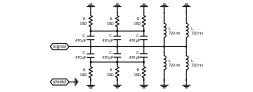
\includegraphics[width=0.9\textwidth]{src/5/figures/shaping_filter_schematic.pdf}
  \caption{Shaping-filter schematic}
  \label{fig:shaping_filter_schematic}
\end{figure}

\begin{figure}[!h]
  \centering
  \includegraphics[width=0.9\textwidth]{src/5/figures/filter.jpg}
  \caption{Assembled shaping-filter}
  \label{pic:shaping_filter_assembled}
\end{figure}

\subsubsection{Absorber}

Near the end of the HMM waveform, the inductor is drawing almost all the incoming \gls{tlp} current.
After 100ns, the current injected by the TLP into the shaping filter and the \gls{dut} becomes null because the cable is completely discharged.
However, the current inside the inductor cannot be stopped instantly.
Without the absorber, the inductor would keep absorbing a non-zero current after the TLP pulse, drawing a negative potential at point A.
To avoid this phenomenom, the absorber completely filters the TLP falling edge at the end of the pulse.
This way, the current through the inductor is softly brought back to 0 by the absorber, effectively eliminating the negative voltage issue.
It also acts as a matched termination for transient events, which is great to eliminate reflections and prevent ringing oscillations.

The schematic of the absorber is given Fig. \ref{fig:absorber_schematic} and a picture of the assembled device is given in Fig. \ref{pic:absorber_filter_assembled}.
The device is constituted of a 50\textOmega{} resistor, in series with a 6.6 nF capacitor.

\begin{figure}[!h]
  \centering
  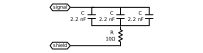
\includegraphics[width=0.7\textwidth]{src/5/figures/absorber_schematic.pdf}
  \caption{Absorber schematic}
  \label{fig:absorber_schematic}
\end{figure}

\begin{figure}[!h]
  \centering
  \includegraphics[width=0.4\textwidth]{src/5/figures/absorber.jpg}
  \caption{Assembled absorber}
  \label{pic:absorber_filter_assembled}
\end{figure}

%\subsubsection{Risetime filter}
%TODO: TODO ?
%Custom design to sustain high voltage
%See Presentation 10 from January 2015
